\documentclass[11pt, a4paper]{report}
\usepackage[utf8]{inputenc}
\usepackage{geometry}
\geometry{a4paper, margin=1in, headheight=15pt}
\usepackage{graphicx}
\usepackage{hyperref}
\usepackage{tikz}
\usetikzlibrary{shapes.geometric, arrows.meta, positioning, calc}
\usepackage{xcolor}
\usepackage{fancyhdr}
\usepackage{titlesec}
\usepackage{tabularx}
\usepackage{enumitem}
\usepackage{microtype} % Improves typography
\renewcommand{\familydefault}{\sfdefault} % Professional sans-serif font

% --- Branding Colors ---
\definecolor{gryorkBlue}{RGB}{14, 42, 71}
\definecolor{gryorkLightBlue}{RGB}{52, 114, 184}
\definecolor{fintechGreen}{RGB}{39, 174, 96}
\definecolor{alertRed}{RGB}{231, 76, 60}
\definecolor{lightGray}{RGB}{245, 247, 250}
\definecolor{darkGray}{RGB}{50, 50, 50}

% --- Hyperlink Formatting ---
\hypersetup{
    colorlinks=true,
    linkcolor=gryorkLightBlue,
    filecolor=gryorkBlue,      
    urlcolor=fintechGreen,
}

% --- Page Style ---
\pagestyle{fancy}
\fancyhf{}
\renewcommand{\headrulewidth}{0.4pt}
\renewcommand{\footrulewidth}{0.4pt}
\rhead{\textcolor{gryorkLightBlue}{\textbf{Fintech Architecture}}}
\lhead{\textcolor{gryorkBlue}{\textbf{Gryork Tech}}}
\cfoot{\textcolor{darkGray}{\thepage}}

% --- Title Formats ---
\titleformat{\chapter}[display]
  {\normalfont\sffamily\bfseries\color{gryorkBlue}}
  {\titlerule[1.5pt]\vspace{2ex}\Large\chaptertitlename\ \thechapter}
  {1ex}
  {\huge}
  [\vspace{1ex}\titlerule]

\titleformat{\section}
  {\normalfont\sffamily\Large\bfseries\color{gryorkBlue}}
  {\thesection}{1em}{}

\titleformat{\subsection}
  {\normalfont\sffamily\large\bfseries\color{gryorkLightBlue}}
  {\thesubsection}{1em}{}

% --- Spacing ---
\setlength{\parskip}{0.5em}
\setlength{\parindent}{0pt}

\begin{document}

% ==========================================
% TITLE PAGE
% ==========================================
\begin{titlepage}
    \centering
    \vspace*{2cm}
    
    {\Huge \bfseries \textcolor{gryorkBlue}{Architecting Trust at Scale} \par}
    \vspace{1cm}
    {\Large \textbf{\textcolor{darkGray}{A Founder's Blueprint for Integrating India Stack,\\Identity, and Account Aggregators into the Gryork Ecosystem}} \par}
    
    \vspace{3cm}
    
    % Concept Diagram
    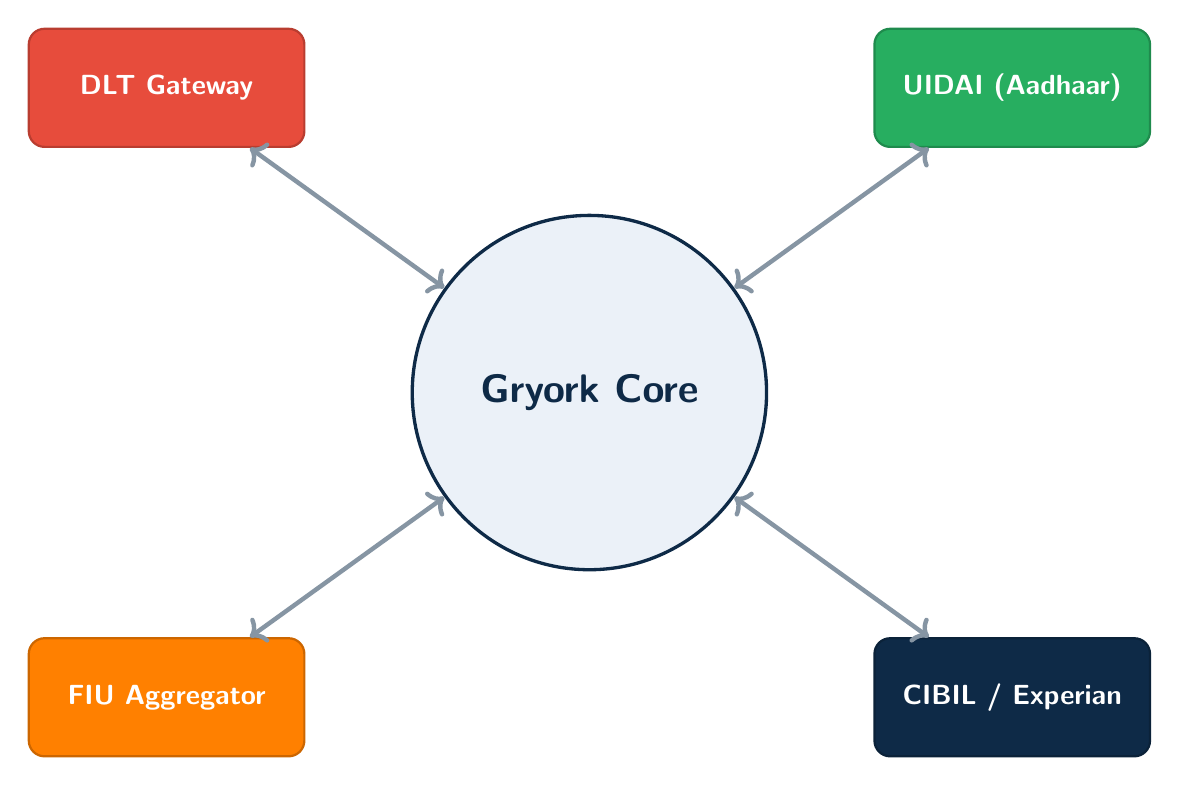
\begin{tikzpicture}[
        node distance=2cm,
        coreNode/.style={circle, draw=gryorkBlue, fill=gryorkLightBlue!10, text=gryorkBlue, minimum size=4.5cm, very thick, align=center, font=\bfseries\Large},
        extNode/.style={rectangle, text=white, minimum width=3.5cm, minimum height=1.5cm, rounded corners=0.2cm, thick, align=center, font=\bfseries}
    ]
        \node[coreNode] (core) {Gryork Core};
        
        \node[extNode, fill=fintechGreen, draw=fintechGreen!80!black, above right=1.5cm and 2cm of core] (uidai) {UIDAI (Aadhaar)};
        \node[extNode, fill=gryorkBlue, draw=gryorkBlue!80!black, below right=1.5cm and 2cm of core] (cibil) {CIBIL / Experian};
        \node[extNode, fill=alertRed, draw=alertRed!80!black, above left=1.5cm and 2cm of core] (otp) {DLT Gateway};
        \node[extNode, fill=orange, draw=orange!80!black, below left=1.5cm and 2cm of core] (aa) {FIU Aggregator};
        
        \draw[<->, ultra thick, gryorkBlue!50] (core) -- (uidai);
        \draw[<->, ultra thick, gryorkBlue!50] (core) -- (cibil);
        \draw[<->, ultra thick, gryorkBlue!50] (core) -- (otp);
        \draw[<->, ultra thick, gryorkBlue!50] (core) -- (aa);
    \end{tikzpicture}
    
    \vfill
    
    \begin{flushright}
        {\large \textbf{Prepared For:} Gryork Executive Team \par}
        {\large \textbf{Date:} \today \par}
        {\large \textbf{Status:} \textcolor{fintechGreen}{Approved for Implementation} \par}
    \end{flushright}
    
\end{titlepage}

\tableofcontents
\newpage

% ==========================================
% CHAPTER 1: EXECUTIVE SUMMARY
% ==========================================
\chapter{Executive Summary}

As the Indian B2B landscape matures, the bar for trust and underwriting is rising exponentially. At Gryork, managing Subcontractors and EPCs via our Next.js portals and monolithic Node.js backend requires more than manual document uploads. Our current \texttt{SubContractor.js} schema relies heavily on manual KYC verifications (where \texttt{panCard}, \texttt{aadhaarCard}, and \texttt{cancelledCheque} images are manually uploaded and evaluated).

This report outlines our strategic transition from \textbf{Manual Verification} to \textbf{India Stack-Native Verification}. By integrating Aadhaar Offline eKYC, Account Aggregator (AA) APIs, automated De-dupe constraints, and Experian/CIBIL APIs, Gryork will reduce onboarding friction by 60\%, drop fraudulent entries to near-zero, and empower instant credit decisions for the CWCRF ledger. 

\textbf{Key Transition Pillars:}
\begin{enumerate}[label=\textbf{\textcolor{gryorkLightBlue}{\arabic*.}}, itemsep=0.3em]
    \item \textbf{Identity Legality:} Migrating to Aadhaar XML and PAN verification APIs to guarantee compliance with Reserve Bank of India (RBI) and UIDAI mandates.
    \item \textbf{Financial Pulse:} Operating as an FIU (Financial Information User) via Sahamati. This connects us directly to Subcontractors' core banking logic, unlocking machine-readable cash flow analysis.
    \item \textbf{Credit Readiness:} Real-time CIBIL and Experian polling for predictive Default modeling.
\end{enumerate}

% ==========================================
% CHAPTER 2: AADHAAR eKYC & OTP ARCHITECTURE
% ==========================================
\chapter{Identity Validation Workflow (JAM Trinity)}

Because direct API access to the UIDAI CIDR is restricted to authorized entities (e.g., banks, telecoms), Gryork will utilize an \textbf{Offline Aadhaar XML} workflow via an authorized empanelled gateway like Setu, Zoop.one, or Digio.

\section{Modern OTP Infrastructure}
OTP delivery for fintech applications in India is strictly governed by the TRAI's DLT (Distributed Ledger Technology) framework to curb spam and SMS fraud. 
\begin{itemize}[itemsep=0.3em]
    \item \textbf{Regulatory Action:} We must officially register Gryork's brand and our transactional SMS templates on a DLT platform (such as JioTrueConnect).
    \item \textbf{Backend Logic:} Our existing Express.js microservice will integrate a Redis cache to store 6-digit SHA-hashed tokens with a strict 180-second TTL (Time To Live), rejecting repeated brute-force attempts.
\end{itemize}

\section{Aadhaar Offline eKYC Architecture}
Below is the technical integration workflow mapping how we will drastically augment the \texttt{SubContractor} data flow.

\begin{figure}[htbp]
\centering
\vspace{0.7cm}
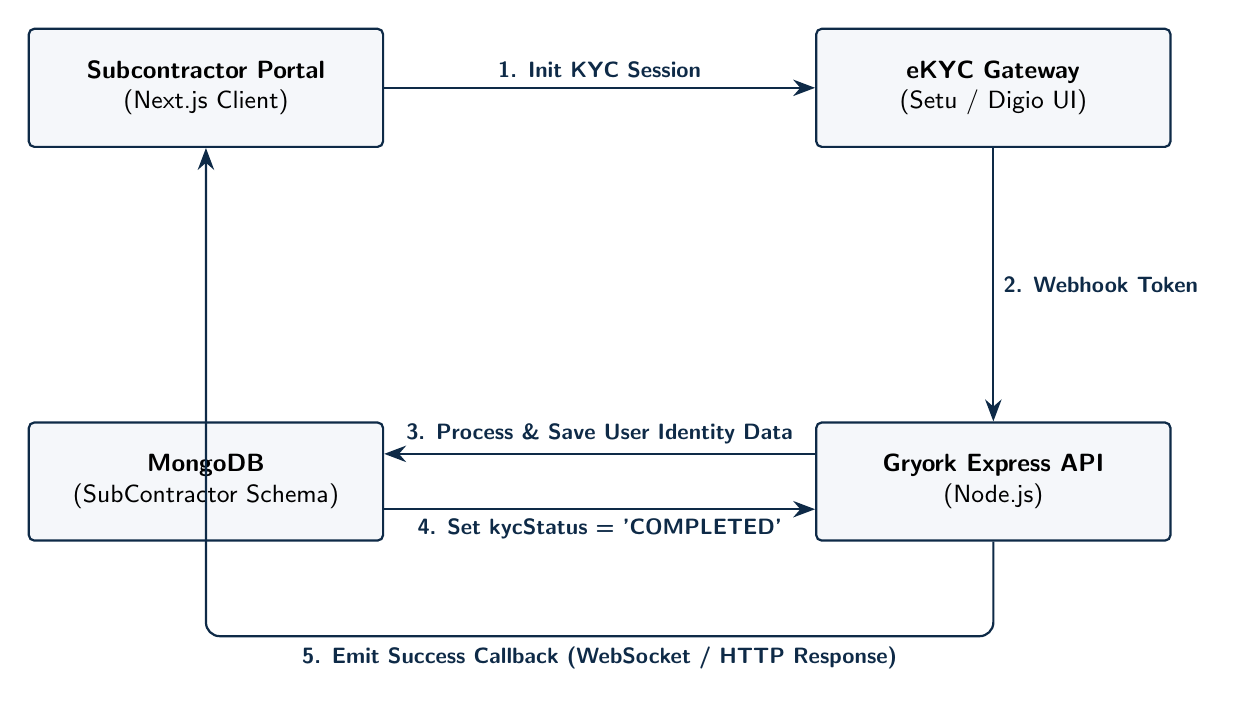
\begin{tikzpicture}[
    box/.style={rectangle, draw=gryorkBlue, fill=lightGray, thick, rounded corners=2pt, align=center, minimum width=4.5cm, minimum height=1.5cm, inner sep=0.2cm, font=\small},
    arrow/.style={-{Stealth[scale=1.2]}, thick, gryorkBlue}
]

% Nodes laid out logically (no overlapping) - Increased X distance for more center space
\node[box] (portal)     at (0, 0) {\textbf{Subcontractor Portal}\\(Next.js Client)};
\node[box] (digilocker) at (10, 0) {\textbf{eKYC Gateway}\\(Setu / Digio UI)};
\node[box] (backend)    at (10, -5) {\textbf{Gryork Express API}\\(Node.js)};
\node[box] (mongo)      at (0, -5) {\textbf{MongoDB}\\(SubContractor Schema)};

% Paths
\draw[arrow] (portal) -- node[above, font=\footnotesize\bfseries, text=gryorkBlue] {1. Init KYC Session} (digilocker);
\draw[arrow] (digilocker) -- node[right, font=\footnotesize\bfseries, text=gryorkBlue, align=center] {2. Webhook Token} (backend);

% Shift lines to prevent overlap
\draw[arrow] ([yshift=10pt]backend.west) -- node[above, font=\footnotesize\bfseries, text=gryorkBlue] {3. Process \& Save User Identity Data} ([yshift=10pt]mongo.east);
\draw[arrow] ([yshift=-10pt]mongo.east) -- node[below, font=\footnotesize\bfseries, text=gryorkBlue] {4. Set kycStatus = 'COMPLETED'} ([yshift=-10pt]backend.west);

\draw[arrow, rounded corners=5pt] (backend.south) -- ++(0,-1.2) -| node[pos=0.25, below, font=\footnotesize\bfseries, text=gryorkBlue] {5. Emit Success Callback (WebSocket / HTTP Response)} (portal.south);

\end{tikzpicture}
\vspace{0.7cm}
\caption{Aadhaar eKYC Data Flow via 3rd Party Gateway}
\end{figure}

% ==========================================
% CHAPTER 3: DE-DUPE & PROFILING LOGIC
% ==========================================
\chapter{Algorithmic De-duplication (De-Dupe)}

Duplicate subcontractor profiles pose massive risks for our CWCRF ledger, potentially allowing blacklisted entities to re-register. Currently, we utilize a basic database index: \texttt{subContractorSchema.index(\{ pan: 1 \});}. It is imperative we transition to a multi-tiered validation matrix.

\section{The Gryork De-Dupe Pipeline}
This automated pipeline will act as a middleware guard before any \texttt{User.create()} or \texttt{SubContractor.create()} resolution:

\begin{enumerate}[label=\textbf{\textcolor{gryorkBlue}{Step \arabic*.}}, itemsep=0.3em]
    \item \textbf{Deterministic Matching (Exact Hit):} Validate exact matches across \texttt{panNumber}, \texttt{gstin}, or the \texttt{vid} (Virtual ID). If matched, trigger a 409 Conflict.
    \item \textbf{Probabilistic Matching (Fuzzy Text):} Utilize Levenshtein distance computations via MongoDB Text Indexes. For example, if "Ritesh Yadav EPC" is registered, an application for "R. Yadav EPC" will be auto-flagged for Ops verification.
    \item \textbf{Contact Overlaps:} Hash comparisons across \texttt{email} strings and \texttt{phone} vectors.
\end{enumerate}

\section{Database Schema Enhancements}
We will extend the \texttt{SubContractor} model with the following audit parameters:
\begin{verbatim}
dedupeFlags: {
    isDuplicate: { type: Boolean, default: false },
    probabilityScore: { type: Number, min: 0, max: 100 },
    matchedEntityId: { 
        type: mongoose.Schema.Types.ObjectId, 
        ref: "SubContractor" 
    }
}
\end{verbatim}

% ==========================================
% CHAPTER 4: CIBIL & ACCOUNT AGGREGATOR
% ==========================================
\chapter{Underwriting \& Trust Engines}

To compute accurate working capital limits, Gryork must ingest the exact financial footprint of the EPC and the Subcontractor. This requires leaving subjective PDF analysis behind and integrating real-time API conduits.

\section{Gryork as an FIU (Account Aggregator)}
Operating as a Financial Information User (FIU) under the Sahamati guidelines allows Gryork to issue a secure "Consent Request" to the Subcontractor. Upon OTP approval, their central bank directly streams their statement data to us as heavily authenticated, machine-readable JSON/XML.

\subsection{Sahamati FIU Architecture}
\begin{figure}[htbp]
\centering
\vspace{0.7cm}
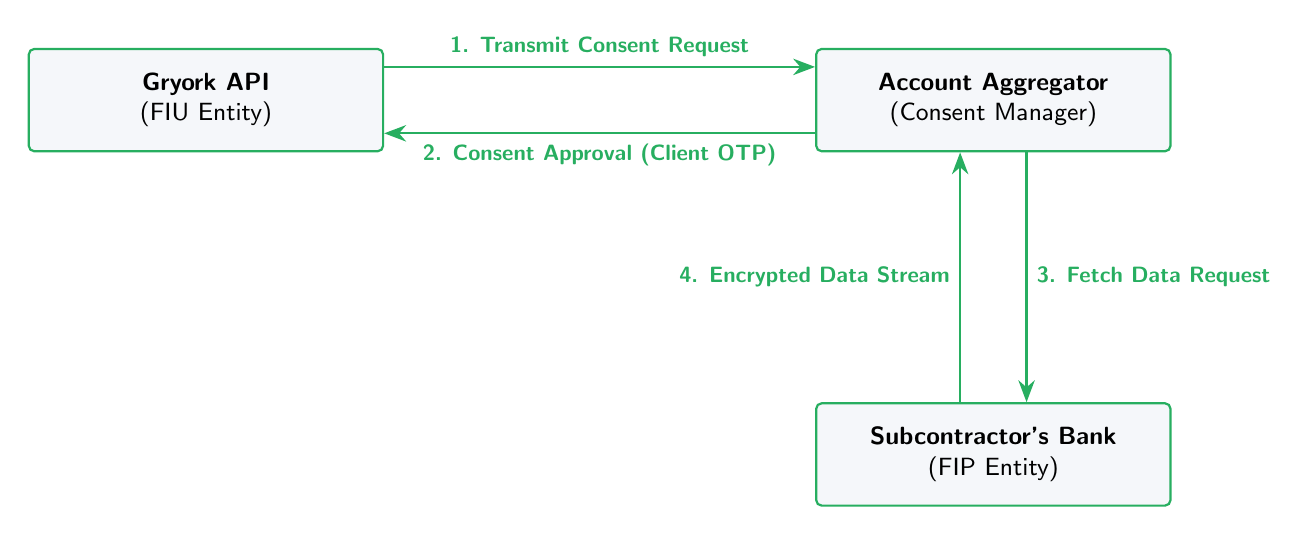
\begin{tikzpicture}[
    box/.style={rectangle, draw=fintechGreen, fill=lightGray, thick, rounded corners=2pt, align=center, minimum width=4.5cm, minimum height=1.3cm, inner sep=0.2cm, font=\small},
    arrow/.style={-{Stealth[scale=1.2]}, thick, fintechGreen}
]

% Increased spacing for second diagram
\node[box] (fiu) at (0, 0)   {\textbf{Gryork API}\\(FIU Entity)};
\node[box] (aa)  at (10, 0)   {\textbf{Account Aggregator}\\(Consent Manager)};
\node[box] (fip) at (10, -4.5) {\textbf{Subcontractor's Bank}\\(FIP Entity)};

% Inter-node paths
\draw[arrow] ([yshift=12pt]fiu.east) -- node[above, font=\footnotesize\bfseries, text=fintechGreen] {1. Transmit Consent Request} ([yshift=12pt]aa.west);
\draw[arrow] ([yshift=-12pt]aa.west) -- node[below, font=\footnotesize\bfseries, text=fintechGreen] {2. Consent Approval (Client OTP)} ([yshift=-12pt]fiu.east);

\draw[arrow] ([xshift=12pt]aa.south) -- node[right, font=\footnotesize\bfseries, text=fintechGreen, align=left] {3. Fetch Data Request} ([xshift=12pt]fip.north);
\draw[arrow] ([xshift=-12pt]fip.north) -- node[left, font=\footnotesize\bfseries, text=fintechGreen, align=right] {4. Encrypted Data Stream} ([xshift=-12pt]aa.south);

\end{tikzpicture}
\vspace{0.7cm}
\caption{Sahamati Account Aggregator Consent \& Data Flow}
\end{figure}

\section{Experian \& CIBIL Integration}
Gryork will invoke the Experian API via an isolated backend Node.js microservice. When a lead profile hits \texttt{status: 'RMT\_PENDING'}, a daemon job retrieves their credit footprint.

\begin{itemize}[itemsep=0.3em]
    \item \textbf{Compliance Guideline:} We will \underline{not} persist the entire detailed credit dataset in plaintext within MongoDB. We will capture and store only the decisive algorithmic artifacts (e.g., Score: \texttt{780}, HighRisk: \texttt{false}) mapped alongside the Experian Trace ID.
\end{itemize}

% ==========================================
% CHAPTER 5: CONCLUSION & ROADMAP
% ==========================================
\chapter{Roadmap to Production}
This architecture will be merged systematically to prevent downtime across the Gryork monorepo network.

\begin{center}
\renewcommand{\arraystretch}{1.5}
\begin{tabularx}{\textwidth}{|>{\columncolor{gryorkBlue!10}\bfseries}l|X|}
\hline
\rowcolor{gryorkBlue}
\textcolor{white}{\textbf{Execution Phase}} & \textcolor{white}{\textbf{Primary Engineering Deliverables}} \\
\hline
Phase 1: Foundation (Weeks 1-3) & DLT Registration, OTP Gateway integration, Next.js UI Auth revamp, and MongoDB Text indexing for Dedupe functions. \\
\hline
Phase 2: Identity (Weeks 4-6) & Aadhaar XML integration. Graceful deprecation of manual OCR PDF reviews in the \texttt{official\_portal}. \\
\hline
Phase 3: Financials (Weeks 7-10) & CIBIL fetch automation, Sahamati FIU module certification, and FIU widget embedding inside \texttt{subcontractor-portal}. \\
\hline
\end{tabularx}
\end{center}

\vspace{1.5cm}
\begin{center}
\large\textit{"This architecture bridges trust and execution, empowering the Gryork ecosystem to scale from thousands to millions of secure operational transactions entirely autonomously."}
\end{center}

\end{document}
